\RequirePackage[l2tabu, orthodox]{nag}
\documentclass{article}

\usepackage[letterpaper, margin=1.3cm]{geometry}
\usepackage{siunitx}
\usepackage{mathtools}
\usepackage{multicol}
\usepackage{amssymb}
\usepackage{mathrsfs}
\usepackage{enumitem}
\usepackage{circuitikz}
\usepackage{booktabs}
\usepackage{multirow}
\usepackage{pdfpages}
\usepackage[outputdir=obj]{minted}

\ctikzset{
    logic ports=ieee,
    logic ports/scale=0.7,
}

\title{ECE 410 Assignment 3}
\author{Michael Kwok}

\begin{document}
\maketitle
\begin{enumerate}
  \item The synthesis tool goes through each condition of the \textit{if-generate} statement until the first valid condition or the (optional) else block is reached during the elaboration step. For the \textit{case-generate} statement, an expression that is computable during elaboration will be calculated to find the matching \textit{when} arm, and that will be the netlist generated for that case.

        if-generate:
        \begin{minted}{vhdl}
gen_loop : FOR i IN 0 TO WID - 1 GENERATE
  adders : IF i > 0 GENERATE
    full : COMPONENT FullAdder PORT MAP(
      A        => A(i),
      B        => B(i),
      carry_in => carry_temp(i - 1),
      sum      => sum(i),
      carry    => carry_temp(i));
  ELSIF i = 0 GENERATE
    half : COMPONENT HalfAdder PORT MAP(
      A     => A(i),
      B     => B(i),
      sum   => sum(i),
      carry => carry_temp(i));
  END GENERATE;
END GENERATE;      
        \end{minted}

        case-generate:
        \begin{minted}{vhdl}
gen : CASE type GENERATE
WHEN RIPPLE => 
  add: ENTITY work.adder(ripple)
    PORT MAP (
      A         => A,
      B         => B,
      carry_in  => carry_in,
      sum       => sum,
      carry_out => carry_out;
    );
WHEN LOOKAHEAD => 
  add: ENTITY work.adder(cla)
    PORT MAP (
      A         => A,
      B         => B,
      carry_in  => carry_in,
      sum       => sum,
      carry_out => carry_out;
    );
WHEN OTHERS => 
  add: ENTITY work.adder(Behavioural)
    PORT MAP (
      A         => A,
      B         => B,
      carry_in  => carry_in,
      sum       => sum,
      carry_out => carry_out;
    );
        \end{minted}

  \item Available microcontrollers might not have the requisite speed to process the data the way the system needs it to, so a custom data processing hardware design might be required, such as navigation guidance systems where the data needs to be processed extremely quickly.

        Power effeciency of more specialized hardware as compared to a general microcontroller is a reason to design bespoke hardware for the task. When the task is known, unused hardware can be disabled, such as turning off the multiplier circuit when the current phase of the task only needs integer rotation, which greatly reduces static power usage of the circuit.

        A design done as custom hardware is likely to be more reliable. Logic circuits are easier to reason and verify formally as compared to programming instructions.

  \item Attached at the end.

  \item By designing the datapath first from the algorithm, the control signals required for each step can be extracted and be used when designing the controller. If the controller was to be designed first, the designer would have to think ahead to avoid creating insufficient controller signals, and having to force the datapath's design around insufficient control signals. There might also be status signals that the controller assumes are required but the datapath might not need. Overall, it could cause an inefficient final design.

  \item
        Top level module:
        \inputminted{vhdl}{src/VectorCounter.vhd}

        Controller:
        \inputminted{vhdl}{src/VectorCounterController.vhd}

        Datapath:
        \inputminted{vhdl}{src/VectorCounterDatapath.vhd}

        Triplet Checker:
        \inputminted{vhdl}{src/TripletChecker.vhd}

        Parity Checker:
        \inputminted{vhdl}{src/ParityChecker.vhd}
\end{enumerate}

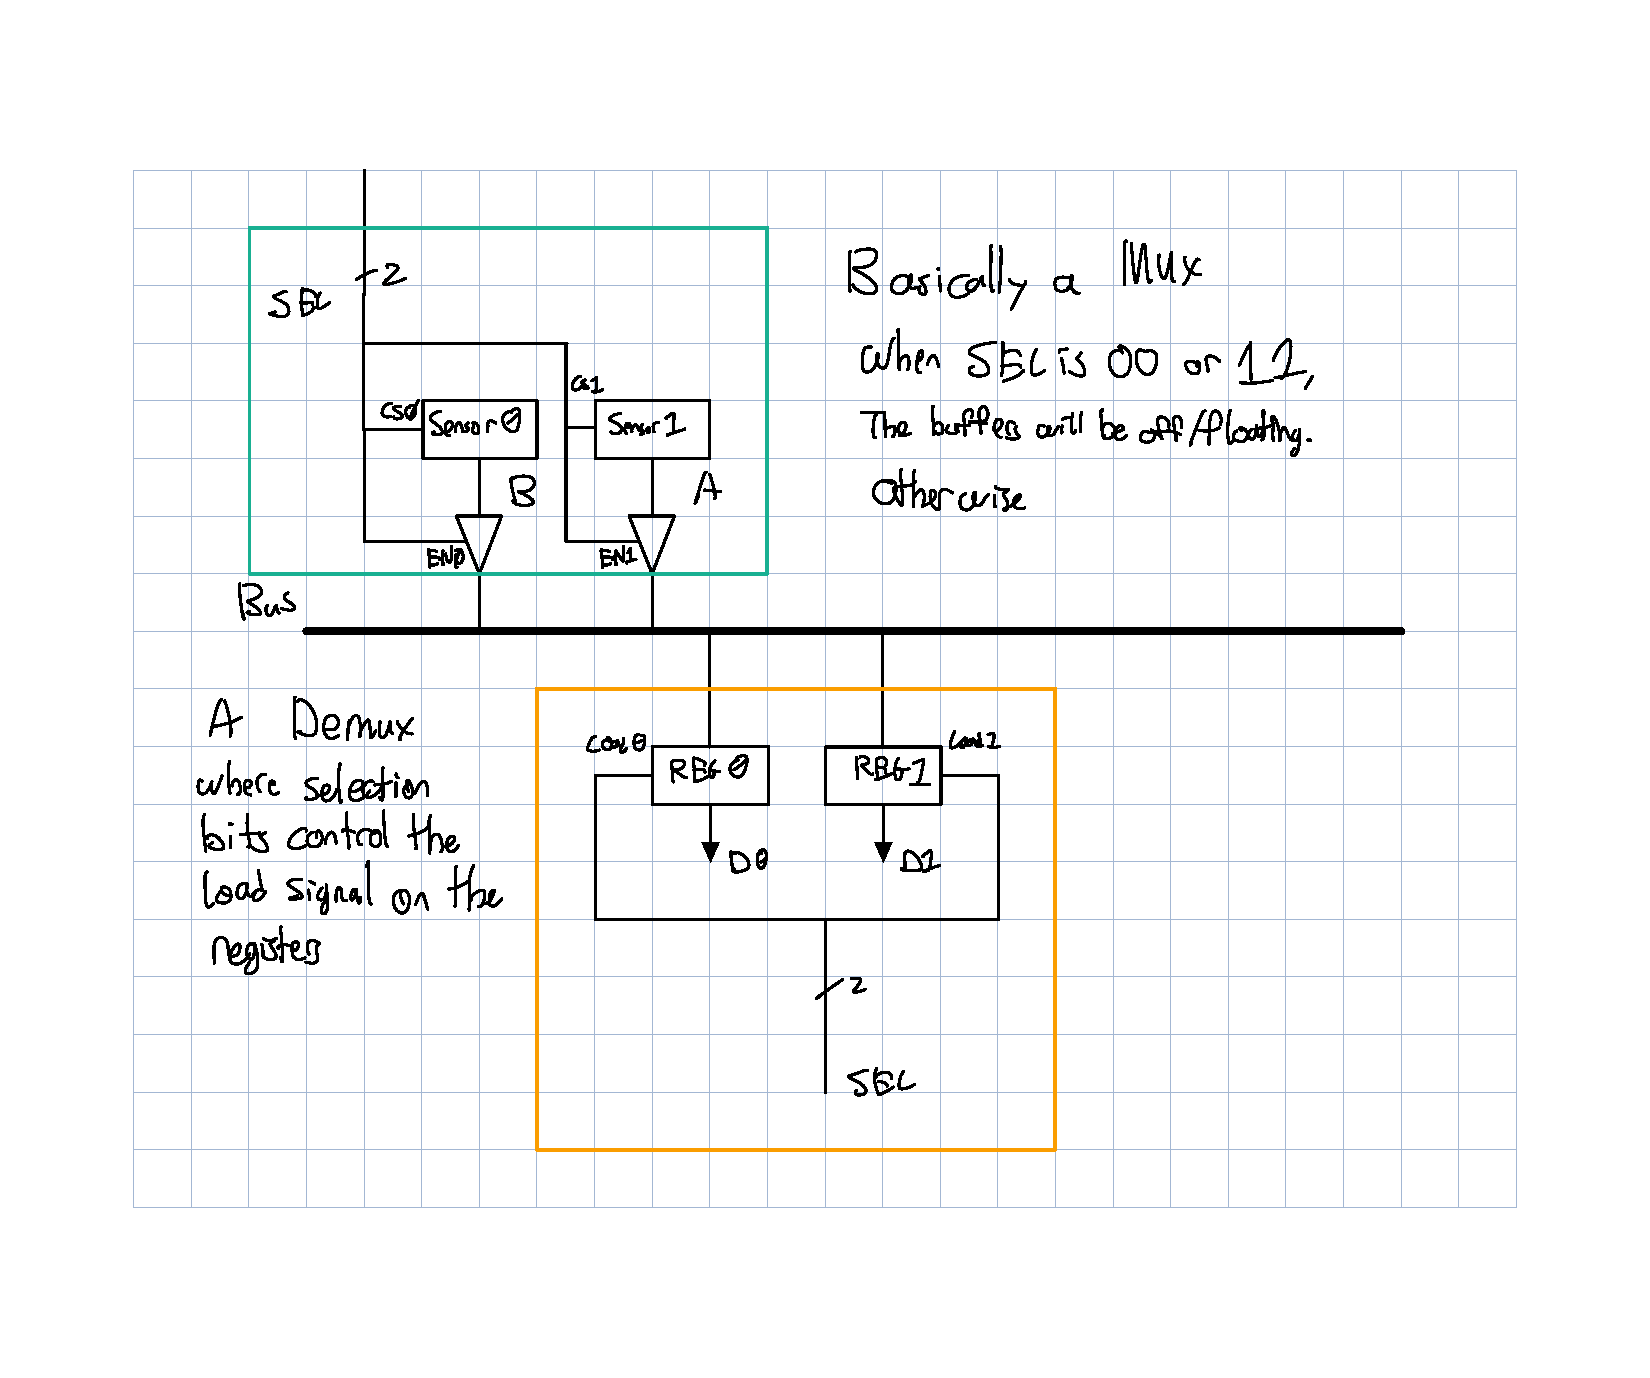
\includepdf[pages=-]{MUX.pdf}

\end{document}
